%%%%%%%%%%%%%%%%%%%%%%%%%%%%%%%%%%%%%%%%%%%%%%%%%%%%%%%%%%%%%%%%%%%%
%% I, the copyright holder of this work, release this work into the
%% public domain. This applies worldwide. In some countries this may
%% not be legally possible; if so: I grant anyone the right to use
%% this work for any purpose, without any conditions, unless such
%% conditions are required by law.
%%%%%%%%%%%%%%%%%%%%%%%%%%%%%%%%%%%%%%%%%%%%%%%%%%%%%%%%%%%%%%%%%%%%

\documentclass[
  digital,     %% The `digital` option enables the default options for the
               %% digital version of a document. Replace with `printed`
               %% to enable the default options for the printed version
               %% of a document.
%%  color,       %% Uncomment these lines (by removing the %% at the
%%               %% beginning) to use color in the printed version of your
%%               %% document
  oneside,     %% The `oneside` option enables one-sided typesetting,
               %% which is preferred if you are only going to submit a
               %% digital version of your thesis. Replace with `twoside`
               %% for double-sided typesetting if you are planning to
               %% also print your thesis. For double-sided typesetting,
               %% use at least 120 g/m² paper to prevent show-through.
  nosansbold,  %% The `nosansbold` option prevents the use of the
               %% sans-serif type face for bold text. Replace with
               %% `sansbold` to use sans-serif type face for bold text.
  nocolorbold, %% The `nocolorbold` option disables the usage of the
               %% blue color for bold text, instead using black. Replace
               %% with `colorbold` to use blue for bold text.
  lof,         %% The `lof` option prints the List of Figures. Replace
               %% with `nolof` to hide the List of Figures.
  lot,         %% The `lot` option prints the List of Tables. Replace
               %% with `nolot` to hide the List of Tables.
]{fithesis4}
%% The following section sets up the locales used in the thesis.
\usepackage[resetfonts]{cmap} %% We need to load the T2A font encoding
\usepackage[T1,T2A]{fontenc}  %% to use the Cyrillic fonts with Russian texts.
\usepackage[
  main=english, %% By using `czech` or `slovak` as the main locale
                %% instead of `english`, you can typeset the thesis
                %% in either Czech or Slovak, respectively.
  english, german, czech, slovak %% The additional keys allow
]{babel}        %% foreign texts to be typeset as follows:
%%
%%   \begin{otherlanguage}{german}  ... \end{otherlanguage}
%%   \begin{otherlanguage}{czech}   ... \end{otherlanguage}
%%   \begin{otherlanguage}{slovak}  ... \end{otherlanguage}
%%
%%
%% The following section sets up the metadata of the thesis.
\thesissetup{
    date        = \the\year/\the\month/\the\day,
    university  = mu,
    faculty     = fi,
    type        = mgr,
    department  = Department of Computer Systems and Communications,
    author      = Bc. Pavol Baran,
    gender      = m,
    advisor     = {RNDr. Lukáš Hejtmánek, Ph.D.},
    title       = {Checkpoint/Restore in Jupyterhub},
    TeXtitle    = {Checkpoint/Restore in Jupyterhub},
    keywords    = {JupyterHub, JupyterLab, Jupyter Notebook, Kubernetes, Checkpoint, Restore, Spawner},
    TeXkeywords = {JupyterHub, JupyterLab, Jupyter Notebook, Kubernetes, Checkpoint, Restore, Spawner},
    abstract    = {TODO: at the end},
    thanks      = {I would like to thank my advisor RNDr. Lukáš Hejtmánek, Ph.D., for his help and guidance, as well as RNDr. Viktória Spišaková for helping me troubleshoot CRIU issues. Lastly, I want to thank my family and friends for supporting me throughout this tough period of my life.},
    bib         = example.bib,
    %% Remove the following line to use the JVS 2018 faculty logo.
    facultyLogo = fithesis-fi,
}
\usepackage{makeidx}      %% The `makeidx` package contains
\makeindex                %% helper commands for index typesetting.
%% These additional packages are used within the document:
\usepackage{paralist} %% Compact list environments
\usepackage{amsmath}  %% Mathematics
\usepackage{amsthm}
\usepackage{amsfonts}
\usepackage{url}      %% Hyperlinks
\usepackage{markdown} %% Lightweight markup
\usepackage{listings} %% Source code highlighting
\lstset{
  basicstyle      = \ttfamily,
  identifierstyle = \color{black},
  keywordstyle    = \color{blue},
  keywordstyle    = {[2]\color{cyan}},
  keywordstyle    = {[3]\color{olive}},
  stringstyle     = \color{teal},
  commentstyle    = \itshape\color{magenta},
  breaklines      = true,
}
\usepackage{floatrow} %% Putting captions above tables
\floatsetup[table]{capposition=top}
\usepackage[babel]{csquotes} %% Context-sensitive quotation marks

%%Does \Cref links
\usepackage{hyperref}
\usepackage{cleveref}

% Only 2 leveled Contents
\addtocontents{toc}{\setcounter{tocdepth}{1}}


% CODE LISTING
\lstdefinelanguage{Go}{
  % Keywords as defined in the language grammar
  morekeywords=[1]{%
    break,default,func,interface,select,case,defer,go,map,%
    struct,chan,else,goto,package,switch,const,fallthrough,%
    if,range,type, continue,for,import,return,var},
  % Built-in functions
  morekeywords=[2]{%
    append,cap,close,complex,copy,delete,imag,%
    len,make,new,panic,print,println,real,recover},
  % Pre-declared types
  morekeywords=[3]{%
    bool,byte,complex64,complex128,error,float32,float64,%
    int,int8,int16,int32,int64,rune,string,%
    uint,uint8,uint16,uint32,uint64,uintptr},
  % Constants and zero value
  morekeywords=[4]{true,false,iota,nil},
  % Strings : "foo", 'bar', `baz`
  morestring=[b]{"},
  morestring=[b]{'},
  morestring=[b]{`},
  % Comments : /* comment */ and // comment
  comment=[l]{//},
  morecomment=[s]{/*}{*/},
  % Options
  sensitive=true
}
\lstset{language=Go,
  basicstyle=\ttfamily\scriptsize,
  keywordstyle=\color{blue}\ttfamily,
  stringstyle=\color{red}\ttfamily,
  commentstyle=\color{green}\ttfamily}

% END CODE


\usepackage[newfloat]{minted}
\usepackage{caption}
\newenvironment{code}{\captionsetup{type=listing}}{}
\SetupFloatingEnvironment{listing}{name=Listing}



\begin{document}
%% The \chapter* command can be used to produce unnumbered chapters:
\chapter*{Introduction}
%% Unlike \chapter, \chapter* does not update the headings and does not
%% enter the chapter to the table of contents. I we want correct
%% headings and a table of contents entry, we must add them manually:
\markright{\textsc{Introduction}}
\addcontentsline{toc}{chapter}{Introduction}

TODO: at the end

\chapter{Project Jupyter}
As this thesis focuses on checkpointing and restoring Jupyter Notebooks within JupyterHub, it begs the question: what even is JupyterHub or Jupyter Notebook? This first part of this chapter provides a brief look into what Jupyter Notebook is and how it is used before examining its next-generation successor, JupyterLab. The second part discusses JupyterHub, deconstructs it into its fundamental pieces, and describes each piece in detail to give a solid foundation of the inner workings of JupyterHub. The last part describes the specific distribution of JupyterHub on which this thesis builds.

Jupyter Notebook, JupyterLab, and JupyterHub all share one thing in common: their umbrella project, Jupyter.
\emph{Project Jupyter is an open-source software project and community that builds software, services, and open standards for interactive computing across dozens of programming languages} \cite{granger2021jupyter}.
Project Jupyter and Jupyter originated from the IPython project, which provided an improved interactive Python shell over the default one \cite{ipython}. The same IPython now serves as the default execution engine (\emph{Kernel}) for Jupyter Notebook.

Nowadays, Jupyter Notebooks are widely used in data science, machine learning, and scientific research for tasks like data analysis, with over ten million notebook documents available on GitHub \cite{granger2021jupyter}. In scientific research, Jupyter Notebooks allow researchers to document experiments, perform simulations, and share reproducible procedures. Educators use Jupyter Notebooks for interactive teaching, enabling students to simultaneously learn coding, mathematics, and data visualization. 
Furthermore, businesses use it to create dashboards and reports, helping them organize and communicate data to support informed decisions.

\section{Jupyter Notebook}
Jupyter Notebook is an open-source application that allows users to easily create and share computational notebooks - documents that combine code, interactive controls, plain language, graphs, and figures, among other visualizations \cite{granger2021jupyter}. Although there exist other projects focused on computation notebooks, such as the proprietary Wolfram Mathematica\footnote{\url{https://www.wolfram.com/mathematica/}}, Jupyter Notebooks gained widespread adoption due to its open-source nature and simplicity.

The ability to create a computational notebook comes from the fact that Jupyter Notebook runs as a web server, providing its user interface in a web browser, through which users can write code with auto-completion, execute the code, as well as provide descriptions or annotate the code using Markdown or LaTeX languages. On the other hand, the ability to share computational notebooks stems from the simple format in which the notebooks are stored \cite{jupyter_notebook}.

\begin{figure}[H]
  \begin{center}
  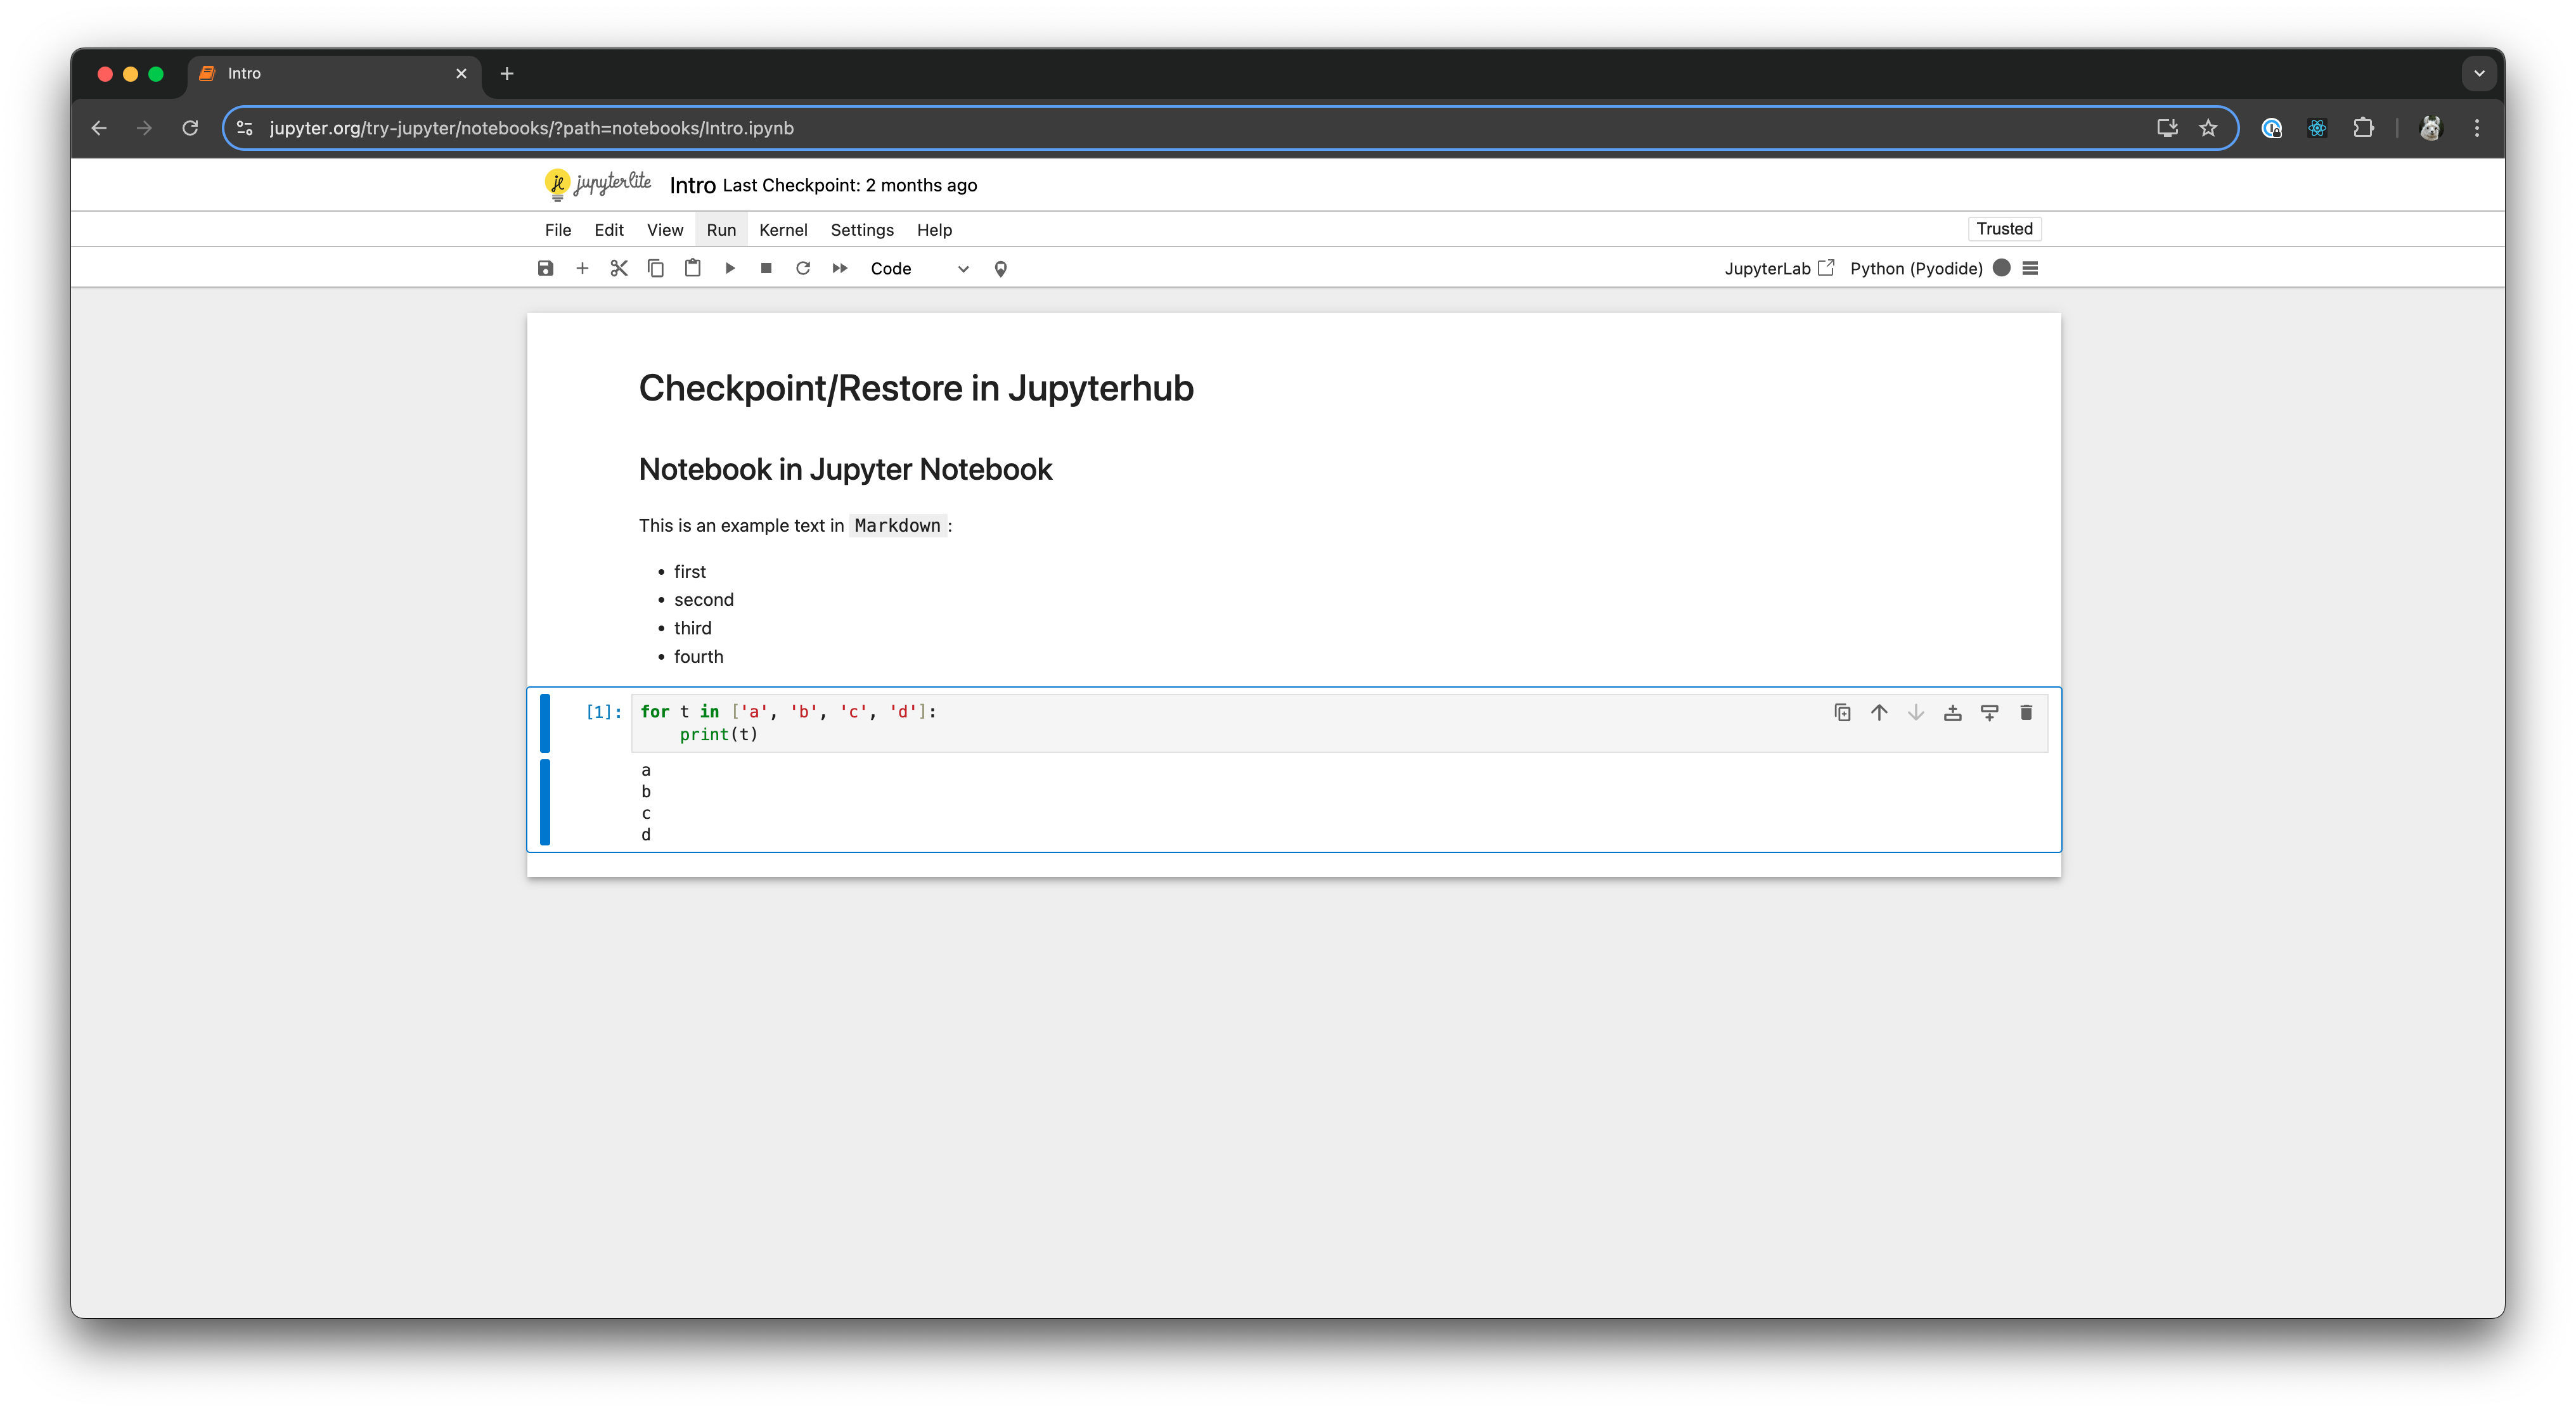
\includegraphics[width=\textwidth]{figures/jupyter-notebook-screenshot.png}
  \end{center}
  \caption{Jupyter Notebook's user interface.}
  \label{fig:jupyter-notebook-screenshot}
\end{figure}

\Cref{fig:jupyter-notebook-screenshot} shows the Notebook's user interface (UI) accessible through a standard web browser. The UI provides common keyboard shortcuts for editing and, as already mentioned, auto-completion of code. However, apart from the functionality of any word processor, the UI allows for the manipulation of cells. These cells are the main building blocks of the notebook document, and there are three types of cells, each serving a specific purpose in structuring the notebook document:

\begin{description}

    \item[Code cell]
    These cells allow for writing and executing code in a particular language, the most common being Python. The actual type of language depends on the \emph{Kernel} with which the Jupyter Notebook server is communicating. The exact mechanism behind the execution of code in the Notebook is out of the scope of this thesis. Nevertheless, there are Kernels for \emph{dozens} of languages, letting users choose from \emph{over a hundred} \cite{perkel2018jupyter} different Kernels.

    \item[Markdown cell]
    These cells are meant for any text describing, explaining, or commenting on the code. Generally, the text in these cells is in Markdown language. However, mathematical notations can also be prescribed using LaTeX \cite{jupyter_notebook}. 
    
    \item[Raw cell]
    Unlike Markdown and Code cells, text in raw cells will be uninterpreted by Jupyter Notebook. Raw cells preserve the content exactly as it is written, which makes them practical in including plain text, scripts in other languages, or data in a specific format that should not alter the notebook's environment.
    
\end{description}

The notebook documents, also commonly referred to as Jupyter Notebooks, or just notebooks 
\footnote{Throughout this thesis, the name \emph{Jupyter Notebook}, will reference only the application itself, not the notebook document that can be created within the application.}
are stored in an open document format based on JSON, with the file itself using \emph{.ipynb} extension. The document contains a complete record of the user's sessions, including the output of the executed code. Since JSON is a plain text format, it allows for version control using Git and easy conversion to other formats, such as HTML, LaTeX, or PDF, using the included tool \emph{nbconvert}. The authors can publish their notebooks to GitHub, share the notebook as an HTML page online, or print the PDF on paper and share it physically \cite{kluyver2016jupyter}. 

% Maybe TODO: Jupyter Notebook has become widely used in AI research communities \url{ https://cdn.aaai.org/ocs/10349/10349-46093-1-PB.pdf} and other academical environments with over milion \url{https://ieeexplore.ieee.org/abstract/document/8816763} notebooks available online.

\section{JupyterLab}

JupyterLab's documentation describes JupyterLab as Jupyter Notebook's \emph{sibling} \cite{jupyter_lab}. However, referring to it as a sibling might give the impression that JupyterLab is merely an alternative to Jupyter Notebook. In reality, JupyterLab represents a significant advancement, offering a more sophisticated and customizable user interface that can be tailored to different use cases. JupyterLab retains the core functionalities of Jupyter Notebook, one of which is the document format. However, it expands significantly upon them by providing a modular, flexible workspace that supports multiple panels and interactive widgets, as seen on \Cref{fig:jupyter-lab-screenshot}. Whereas Jupyter Notebook's user interface (\Cref{fig:jupyter-notebook-screenshot}) centers around one notebook document, JupyterLab resembles more of an integrated development environment (IDE), with file browser on the hand left side and a variable inspector on the right.

\begin{figure}[H]
  \begin{center}
  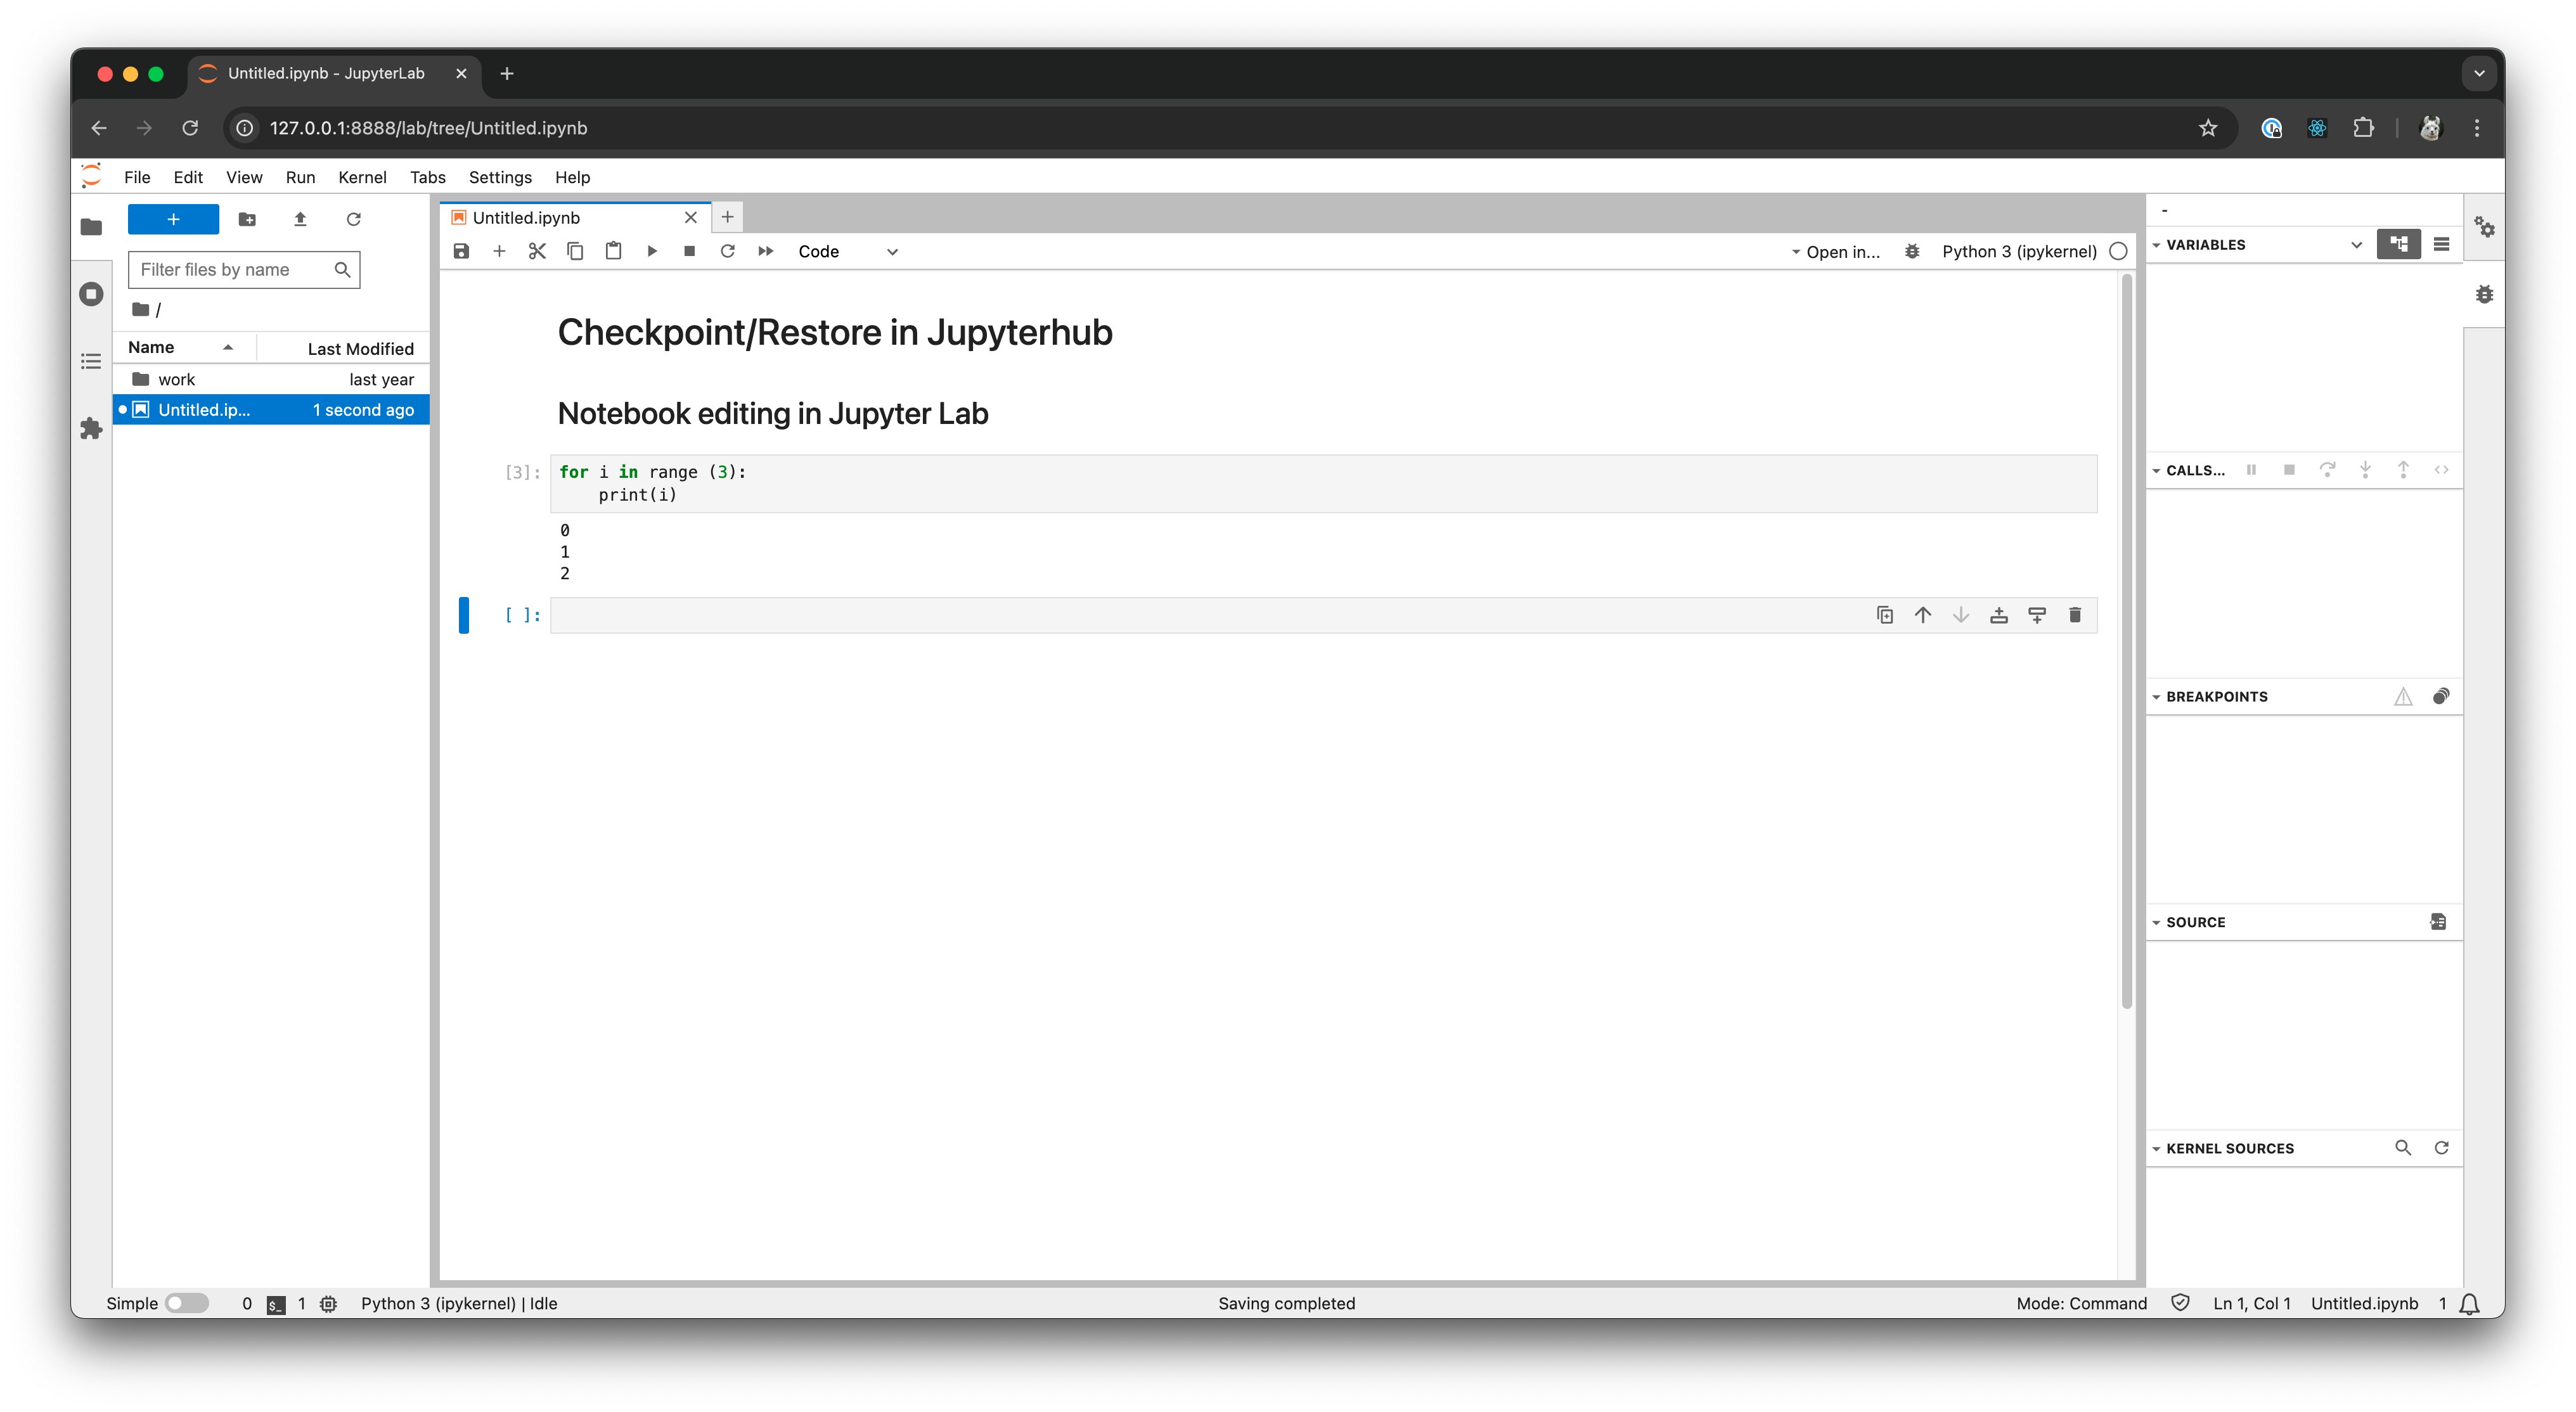
\includegraphics[width=\textwidth]{figures/jupyter-lab-extended-screenshot.png}
  \end{center}
  \caption{JupyterLab's user interface.}
  \label{fig:jupyter-lab-screenshot}
\end{figure}

All this does not negate the fact that some individuals still prefer the comparably simplified interface of Jupyter Notebook or do not see the value in upgrading. Moreover, as JupyterLab supports the same \emph{.ipynb} document format, and the initial versions depended on the installation of Notebook; it is not uncommon, in the community and documentation, to refer to JupyterLab as Jupyter Notebook instead. Consequently, since JupyterHub (\Cref{sec:jupyterhub}) supports both JupyterLab and Jupyter Notebook, this thesis will, henceforth, adopt the term Jupyter Notebook exclusively.

\section{JupyterHub}
\label{sec:jupyterhub}
Jupyter Notebook was initially designed for single-user environments. However, as Jupyter Notebook's popularity rose among researchers, data analysts, and academics, such did the need for a way to quickly deploy Jupyter Notebooks for multiple users in a centralized environment without requiring each user to install Jupyter Notebook. In other words, \emph{IT support for 800 students, helping them debug why the installation on their laptop is not working; that's simply infeasible} \cite{perkel2018jupyter}.

JupyterHub addressed this need by providing a \emph{multi-user Hub that creates, manages, and proxies multiple instances of the single-user Jupyter notebook server}, which allows it to be used in \emph{a class of students, a corporate data science group, or a scientific research group} \cite{jupyterhub}. Simply put, JupyterHub takes the single-user Jupyter Notebook and adds a layer of functionality on top, providing user management and control over the running environment of the Notebooks.

To account for different use cases, serving Jupyter Notebooks to a few as well as hundreds and thousands of users, JupyterHub comes in two distinct distributions:
\begin{description}

    \item[The Littlest JupyterHub (TLJH)]
    Intended primarily for educators teaching small classes of ten to at most a hundred students. The distribution runs on a single server without any containerization technology such as Docker or Kubernetes and intends to provide as simple as possible installation and configuration setup for JupyterHub \cite{littlest_jupyterhub}.

    \item[Zero to JupyterHub with Kubernetes (Z2JH)]
    This distribution runs in Kubernetes, with many of its components running in separate containers, which allow it to dynamically scale up or down depending on the required resources and user demand. By utilizing several Kubernetes Nodes, the distribution can serve even a thousand users \cite{jupyterhub}. This thesis builds upon Z2JH; therefore, \Cref{sec:z2jh} provides a more detailed look into this distribution.
    
\end{description}

Although using one of the distributions gives some assurance of scalability, it is not the only way to run JupyterHub. JupyterHub can be run as any Python application and configured to use specific \emph{Authenticator, Spawner, and Services} (see \Cref{subsec:jupyterhub:architecture}) based on a particular use-case needed to fulfill. The unofficial distribution, \emph{JupyterHub the hard way}\footnote{\url{https://github.com/jupyterhub/jupyterhub-the-hard-way/blob/master/docs/installation-guide-hard.md}}, provides a thorough walk-through for setting up JupyterHub from scratch.


\section{JupyterHub's Architecture}
\label{subsec:jupyterhub:architecture}
JupyterHub comprises several subsystems as depicted on \Cref{fig:jupyter-hub-arch}, many of which have multiple implementations, enabling administrators to pick and choose the best fit for their specific use case, such as different Spawners, Authenticators, and Services. The following subsections provide a brief look into the most significant components.

\begin{figure}[H]
  \begin{center}
  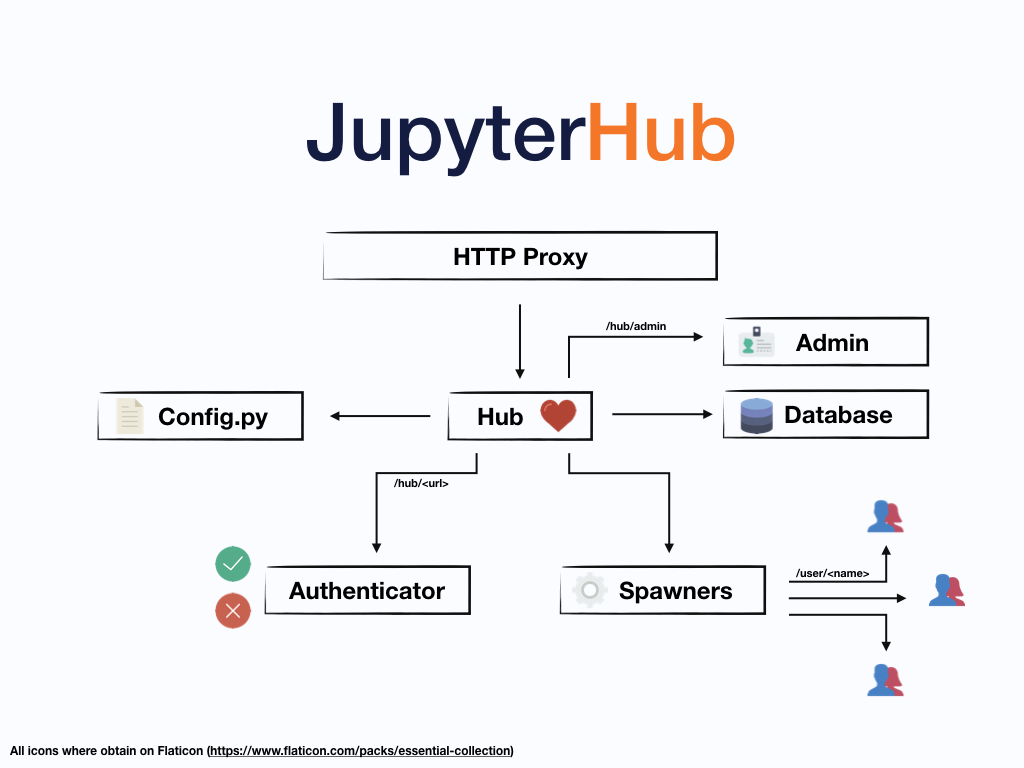
\includegraphics[width=\textwidth]{figures/jupyer-hub-architecture.jpeg}
  \end{center}
  \caption{High level architecture of JupyterHub \cite{jupyterhub}. TODO: maybe replace with custom}
  \label{fig:jupyter-hub-arch}
\end{figure}

\subsection{Hub}
Hub is the central piece connecting all the components. Nevertheless, the end-user only interacts with Hub briefly during login authentication and initialization or shutdown of Jupyter Notebooks. Hub's role is orchestrational in that it starts and stops the Proxy and Services processes, instructs Spawner when to spawn or remove Notebooks, keeps track of users, and delegates authentication of users to the Authenticator.

\subsection{Proxy}
The Proxy, specifically reverse Proxy, serves as an ingress to JupyterHub. Each connection to JupyterHub and, thereby, to the spawned Notebooks goes through the Proxy. This implies that both the Hub and all Notebook applications have to be reachable by the Proxy\cite{jupyterhub_arch}.

When a user connects to JupyterHub for the first time, the Proxy forwards the connection to the Hub. Hub then delegates user authentication to the Authenticator, and only when the user is authenticated does the Hub instruct the Spawner to spawn the Jupyter Notebook. Once the Notebook is up and running, the Hub will update the routing table in the Proxy to forward connections from the specific user\footnote{user's session is tracked using a cookie.} to the spawned Notebook. Afterward, the Proxy forwards each connection of this specific user directly to the Notebook until the user's credentials expire and the whole flow is repeated, except if the Notebook is already running, it does not need to be spawned again.

Hub will start the Proxy as a separate process and stop it on shutdown if it is not configured otherwise. The Proxy can be configured to run entirely separately. Such configuration would allow users to continue using their Notebooks for a certain time, even in case of Hub's unexpected termination \cite{jupyterhub_arch}.

\subsection{Authenticator}
\label{subsec:jupyterhub:authenticator}

Whenever Hub needs to authorize a user's connection or request, it delegates this task to the Authenticator. The Authenticator serves as an interface between Hub and a user management system, allowing validation of user credentials and management of user accounts to be decoupled from JupyterHub. Specifically, Authenticator is part of Hub's codebase, a Python class that can be extended to provide desired functionality.

To keep track of which Notebook belongs to which user, among other tasks, the Hub has to record information about users in a database outside the Authenticator class. Even so, the Hub stores only the data relevant to the user's role and activities in JupyterHub and does not store the users themselves. The management of users, which users exist, and how users login is left up to the Authenticator \cite{jupyterhub_arch}.

Many Authenticator implementations available delegate the user management to a third-party identity provider through OAuth (OAuthenticator), LDAP (ldapauthenticator), or the PAMAuthenticator included in JupyterHub by default, which utilizes the PAM mechanism in Linux to authenticate users. One exception to that is the NativeAuthenticator, which, in fact, stores and validates its own usernames and passwords, effectively managing all users within JupyterHub only. The other exception is the DummyAuthenticator, which, mainly for testing purposes but not only, allows any user to log in \cite{jupyterhub_arch}.

\subsection{Spawner}
Similar to how Authenticator is an interface between Hub and the user management system, the Spawner is an interface between Hub and the running environment of Notebooks. Like Authenticator, Spawner is a Python class in Hub's codebase and has multiple implementations deciding where and how Jupyter Notebooks should be spawned. 

To define itself as Spawner, the Python class needs to be able to perform three actions \cite{jupyterhub_spawner}:
\begin{itemize}
  \item start a Jupyter Notebook
  \item poll whether a Jupyter Notebook is still running
  \item stop a Jupyter Notebook
\end{itemize}
These actions map one-to-one to the class's \emph{start}, \emph{poll}, and \emph{stop} methods. Additionally, as it should be possible for the Hub to stop without affecting the Notebooks, the Spawner can take advantage of two methods, allowing it to persist its internal state across restarts. Hub will call the \emph{load\_state} method for a Spawner to restore its object properties from the state in the database, and \emph{get\_state} to get the internal state of the Spawner to be persisted \cite{jupyterhub_spawner}.

By default, JupyterHub uses the LocalProcessSpawner to spawn Notebooks as local processes, which, however, does not work on Windows. Fortunately, there are many other Spawner implementations, with the notable ones being:
\begin{description}

    \item[DockerSpawner] Capable of spawning Notebooks in Docker containers on the same machine or using DockerSwarm for spawning Notebooks on remote machines \cite{jupyterhub_spawner}. The Spawner can utilize Docker's API and limit the Notebook's allowed CPU and memory usage.
    
    \item[SystemdSpawner]
    Enables to spawn Notebooks using \emph{systemd} the \emph{system and service manager} \cite{systemd} for Linux. Similarly to DockerSpawner, it allows the CPU and memory to be limited for each Notebook. \textbf{The Littlest JupyterHub} distribution uses Spawner, which is based on SystemdSpawner.

    \item[SSHSpawner]
    Can be used to spawn Notebooks on a remote server through SSH. However, it seems that the repository of this Spawner\footnote{https://github.com/NERSC/sshspawner} is no longer actively maintained.

    \item[KubeSpawner]
    Allows spawning Notebooks as Kubernetes Pods and, therefore, can utilize the full potential of Kubernetes API, which implies that JupyterHub must be running in the Kubernetes cluster. This is the Spawner that the \textbf{Zero to JupyterHub with Kubernetes} distribution uses, and as such, this thesis is extending this Spawner with checkpoint and restore capabilities (\Cref{chap:checkpoint_spawner}).
    
\end{description}


\subsection{Services}
\label{subsec:jupyterhub:services}
Services are yet another way JupyterHub can be customized or extended. In the context of JupyterHub, a Service is defined \emph{as something (usually a process) that can interact with the Hub's REST API} \cite{jupyterhub_service}.

JupyterHub recognizes two types of Services. The first type, \textbf{Hub-Managed Service}, are services that are started as a sub-process of Hub and managed directly by Hub. The Hub takes responsibility for starting with a configured command and environment variables, stopping when requested or when the Hub stops, and restarting them when they unexpectedly terminate. The second type, \textbf{Externally-Managed Services}, are independent services that are not directly controlled by the Hub but still need to interact with it. In this case, the Service does not need to be a process; it might be any application. Both types of Services can be specified in JupyterHub's configuration file. However, only Externally-Managed Services can be added or removed at runtime \cite{jupyterhub_service}.

Adding a Service to JupyterHub can have three benefits. Firstly, the Service obtains an API token that it can use to call JupyterHub's REST API with configured permissions. The second benefit is that JupyterHub's Proxy can forward user requests to the Service, thus exposing the Service to the internet or other networks. Lastly, the Service can utilize Hub's authentication mechanism to be accessible only if the user's permissions allow him to.

\subsection{Configuration}
\label{subsec:jupyterhub:configuration}

To configure and customize all the components described, JupyterHub is set up to consume the traitlets\footnote{\url{https://github.com/ipython/traitlets}} configuration file, usually referred to as \emph{jupyterhub\_config.py}.

\begin{code}
\captionof{listing}{JupyterHub's configuration file jupyterhub\_config.py. Maybe TODO: syntax highlight}
\label{lst:jupyterhub:config}
\begin{minted}{yaml}
c.JupyterHub.ip = '0.0.0.0'
c.JupyterHub.port = 8000 
c.JupyterHub.authenticator_class = \ 
    'jupyterhub.auth.PAMAuthenticator'
c.JupyterHub.spawner_class = \
    'jupyterhub.spawner.LocalProcessSpawner'
\end{minted}
\end{code}

The \Cref{lst:jupyterhub:config} shows an example configuration of JupyterHub, setting the IP address and port the Proxy will listen on and specifying the implementation classes of Authenticator and Spawner.

\section{Zero to JupyterHub with Kubernetes}
\label{sec:z2jh}

Initial work on the Zero to JupyterHub with Kubernetes distribution came out of \textbf{Data 8: The Foundations of Data Science
} course at the University of California, Berkeley \cite{z2jh_uc_berkeley}. The idea behind it was to take full advantage of the inherent auto-scaling capabilities of Kubernetes, to be able to serve Jupyter Notebooks to a group of hundreds of people simultaneously, and afterward be able to scale down without having to delete the whole JupyterHub distribution.

Z2JH can be installed on a self-hosted Kubernetes cluster or a cluster managed by one of the public cloud providers like Google or AWS, using Helm chart
\footnote{\emph{A packaged collection of files comprising all of the resources required to manage and deploy an application on a Kubernetes cluster} \cite{helm_charts}}. Similarly to the \emph{jupyterhub\_config.py} described in \Cref{subsec:jupyterhub:configuration}, the installation can be customized using a Helm configuration file, which is referred to as \emph{config.yaml} by Z2JH's documentation \cite{jupyterhub_z2jh_config}, whereas in general it is referred to as the \emph{values file} or \emph{values.yaml} \cite{helm_charts}. In addition to configuring JupyterHub itself, the values file allows the customization of the deployment on the Cluster by defining settings for underlying Kubernetes resources, thus enabling administrators to fine-tune how JupyterHub operates within the Cluster.

\subsection{Architecture}
Many of the principles that apply for \emph{vanilla} JupyterHub apply for Z2JH as well. For example, Z2JH can be configured to use any of the Authenticators described in \Cref{subsec:jupyterhub:authenticator}. Furthermore, Services can be added to JupyterHub the same way described in \Cref{subsec:jupyterhub:services}.

Three main differences are consequential enough to mention. First, the Hub, Proxy, and single-user Notebooks run within separate Kubernetes Pods. This means the communication between the components no longer goes through \emph{localhost} but must be routed based on Pod IP addresses. The second difference is that the distribution contains additional optional components whose purpose is to utilize the cluster resources to a maximum extent. These components include the \emph{continuous-image-puller} whose sole responsibility is to pull Notebook's container image on a newly joined Node in Cluster so that users do not have to wait for it when a Notebook is scheduled on such a Node \cite{jupyterhub_optimizations}. Last but not least, the distribution is designed to work with KubeSpawner, which spawns Jupyter Notebooks as Kubernetes Pods, monitors them, and takes care of deleting them once requested.

\section{KubeSpawner}
\label{sec:kubespawner}
Just like any other Spawner, the KubeSpawner has to be able to execute three actions to work as a Spawner. Start a Jupyter Notebook, poll if it is still running, and stop the Notebook.

When KubeSpawner is requested to spawn a Notebook, it creates a Kubernetes Pod using Python's Kubernetes client. Even though this task might seem straightforward, the KubeSpawner has to do some work before that. Depending on the configuration of KubeSpawner, which significantly affects how the Notebook Pod manifest will look, KubeSpawner might have to create Kubernetes Namespace, Persistent Volume Claim, Secret, and Service\footnote{In the context of Kubernetes Services, not JupyterHub type of Service.}.
Only after can KubeSpawner create the Pod.

For polling, KubeSpawner utilizes an internal object called \emph{Reflector}, specifically \emph{PodReflector}. The job of the Reflector is to \emph{reflect} the state of Cluster, specifically the state of Pods in the Cluster. With the help of Python's Kubernetes client, it does so by watching Pod changes in the Cluster and recording the changes in memory. When KubeSpawner is asked by the Hub if a Notebook is still running, KubeSpawner looks into memory to see if the Pod status shows that it is running and responds adequately.

Stopping a Notebook is a comparatively simple task for KubeSpawner. It requests the removal of the Pod using the Kubernetes client and then waits until PodReflector signals that the Pod has been deleted.


\chapter{Checkpoint/Restore in Userspace}

\section{Checkpoint/Restore in container runtimes}

\section{Checkpoint/Restore in Kubernetes}

\chapter{Checkpoint/Restore of Jupyter Notebooks in Kubernetes}

\section{Architecture}

\chapter{Checkpointer}
\label{chap:checkpointer}

\chapter{CheckpointSpawner}
\label{chap:checkpoint_spawner}


\chapter{Deployment}

\chapter{Future work}
TODO: approx 1-2 page

e.g. about security 

\chapter{Conclusion}
TODO: approx 1 page

  \printbibliography[heading=bibintoc] %% Print the bibliography.

\chapter{Inserting the index}
After using the \verb"\makeindex" macro and loading the
\texttt{makeidx} package that provides additional indexing
commands, index entries can be created by issuing the \verb"\index"
command. \index{dummy text|(}It is possible to create ranged index
entries, which will encompass a span of text.\index{dummy text|)}
To insert complex typographic material -- such as $\alpha$
\index{alpha@$\alpha$} or \TeX{} \index{TeX@\TeX} --
into the index, you need to specify a text string, which will
determine how the entry will be sorted. It is also possible to
create hierarchal entries. \index{vehicles!trucks}
\index{vehicles!speed cars}

After typesetting the document, it is necessary to generate the
index by running
\begin{center}%
  \texttt{texindy -I latex -C utf8 -L }$\langle$\textit{locale}%
  $\rangle$\texttt{ \jobname.idx}
\end{center}
from the command line, where $\langle$\textit{locale}$\rangle$
corresponds to the main locale of your thesis -- such as
\texttt{english}, and then typesetting the document again.

The \texttt{texindy} command needs to be executed from within the
directory, where the \LaTeX\ source file is located. In Windows,
the command line can be opened in a directory by holding down the
\textsf{Shift} key and by clicking the right mouse button while
hovering the cursor over a directory. Select the \textsf{Open Command
Window Here} option in the context menu that opens shortly
afterwards.

With online services -- such as Overleaf -- the commands are
executed automatically, although the locale may be erroneously
detected, or the \texttt{makeindex} tool (which is only able to
sort entries that contain digits and letters of the English
alphabet) may be used instead of \texttt{texindy}. In either case,
the index will be ill-sorted.

  \makeatletter\thesis@blocks@clear\makeatother
  \phantomsection %% Print the index and insert it into the
  \addcontentsline{toc}{chapter}{\indexname} %% table of contents.
  \printindex


\appendix %% Start the appendices.
\chapter{An appendix}
Here you can insert the appendices of your thesis.

\end{document}
